\chapter{Design e Implementazione del Controllore di Tracking} \label{chap:tracking}
\usetikzlibrary{shapes.geometric, arrows.meta, positioning}

Questo capitolo affronta il Punto 2 del progetto: la progettazione e validazione di un controllore per l'inseguimento di traiettoria (tracking problem). Come richiesto dalle specifiche, è stato sviluppato un controllore a libera scelta capace di annullare l'errore di posizionamento rispetto a un riferimento tempo-variante.

\section{Strategia di Controllo}

\subsection{Scelta del Controllore: Feedback Linearization}
Per risolvere il problema del tracking su traiettorie curvilinee complesse, è stata adottata la tecnica della \textit{Feedback Linearization} (linearizzazione esatta tramite retroazione). A differenza di un semplice controllore proporzionale (P) che soffrirebbe di ritardi su percorsi curvi, questo approccio compensa le non-linearità del modello cinematico.

Definito l'errore nel sistema di riferimento globale \( e = z_{ref} - z \), la legge di controllo è strutturata in due stadi:
\begin{enumerate}
    \item \textbf{Anello Esterno (Lineare):} Calcola le velocità virtuali \( v, \omega \) necessarie per stabilizzare l'errore:
    \begin{align}
        v_{des} &= \dot{x}_{ref}\cos\theta + \dot{y}_{ref}\sin\theta + k_x e_x \cos\theta + k_y e_y \sin\theta \\
        \omega_{des} &= \dot{\theta}_{ref} + k_\theta e_\theta
    \end{align}
    \item \textbf{Anello Interno (Inversione):} Mappa le velocità virtuali sulle velocità reali delle ruote \( u_1, u_2 \) invertendo la matrice cinematica (Eq. 7 delle specifiche):
    \begin{equation}
        \begin{bmatrix} u_1 \\ u_2 \end{bmatrix} = 
        \begin{bmatrix} \frac{1}{r_1} & \frac{l}{2r_1} \\ \frac{1}{r_2} & -\frac{l}{2r_2} \end{bmatrix}
        \begin{bmatrix} v_{des} \\ \omega_{des} \end{bmatrix}
    \end{equation}
\end{enumerate}

\subsection{Gestione della Saturazione}
Per garantire il realismo della simulazione, è stato introdotto un blocco di saturazione sugli attuatori. I motori sono limitati a \( u_{max} = \pm 25 \) rad/s. Questo valore è stato dimensionato per garantire che, alla velocità nominale di crociera richiesta dalla traiettoria (circa 15 rad/s), il controllore abbia ancora un margine di \( \pm 10 \) rad/s per effettuare le correzioni.

\section{Schema a Blocchi}
L'architettura del sistema di controllo è stata definita prima a livello logico e poi implementata in ambiente Simulink.

\begin{figure}[h]
    \centering
    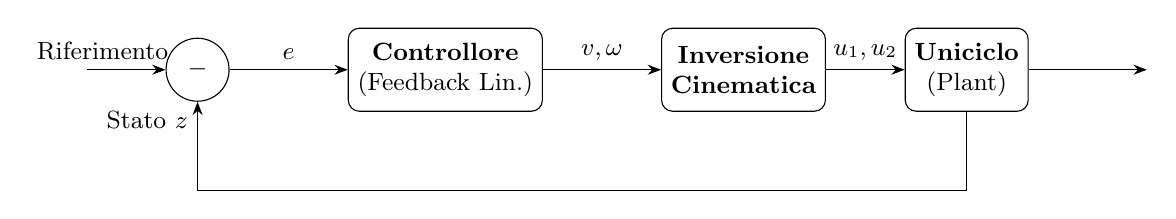
\begin{tikzpicture}[
        auto, 
        node distance=2.5cm, 
        >=Stealth, 
        every node/.style={font=\small},
        block/.style={draw, rectangle, rounded corners, minimum height=3em, minimum width=4em, align=center, fill=white},
        sum/.style={draw, circle, minimum size=0.8cm, inner sep=0pt},
        input/.style={coordinate},
        output/.style={coordinate}
    ]
        % Nodi
        \node [input, name=input] {};
        \node [sum, right=1cm of input] (sum) {};
        \node at (sum) {$-$}; 
        
        \node [block, right=1.5cm of sum] (controller) {\textbf{Controllore} \\ (Feedback Lin.)};
        \node [block, right=1.5cm of controller] (inv_kin) {\textbf{Inversione} \\ \textbf{Cinematica}};
        \node [block, right=1cm of inv_kin] (plant) {\textbf{Uniciclo} \\ (Plant)};
        \node [output, right=1.5cm of plant] (output) {};
        
        % Connessioni
        \draw [->] (input) -- node[above, pos=0.2] {Riferimento} (sum);
        \draw [->] (sum) -- node[above] {\(e\)} (controller);
        \draw [->] (controller) -- node[above] {\(v, \omega\)} (inv_kin);
        \draw [->] (inv_kin) -- node[above] {\(u_1, u_2\)} (plant);
        \draw [->] (plant) -- node[name=y] {} (output);
        
        % Feedback
        \draw [->] (plant.south) -- ++(0,-1.0) -| node[pos=0.9, left] {Stato \(z\)} (sum.south);
    \end{tikzpicture}
    \caption{Schema a blocchi logico del controllo implementato.}
    \label{fig:control_scheme}
\end{figure}

\begin{figure}[h]
    \centering
    % Inserisci qui il percorso corretto della tua immagine Simulink
    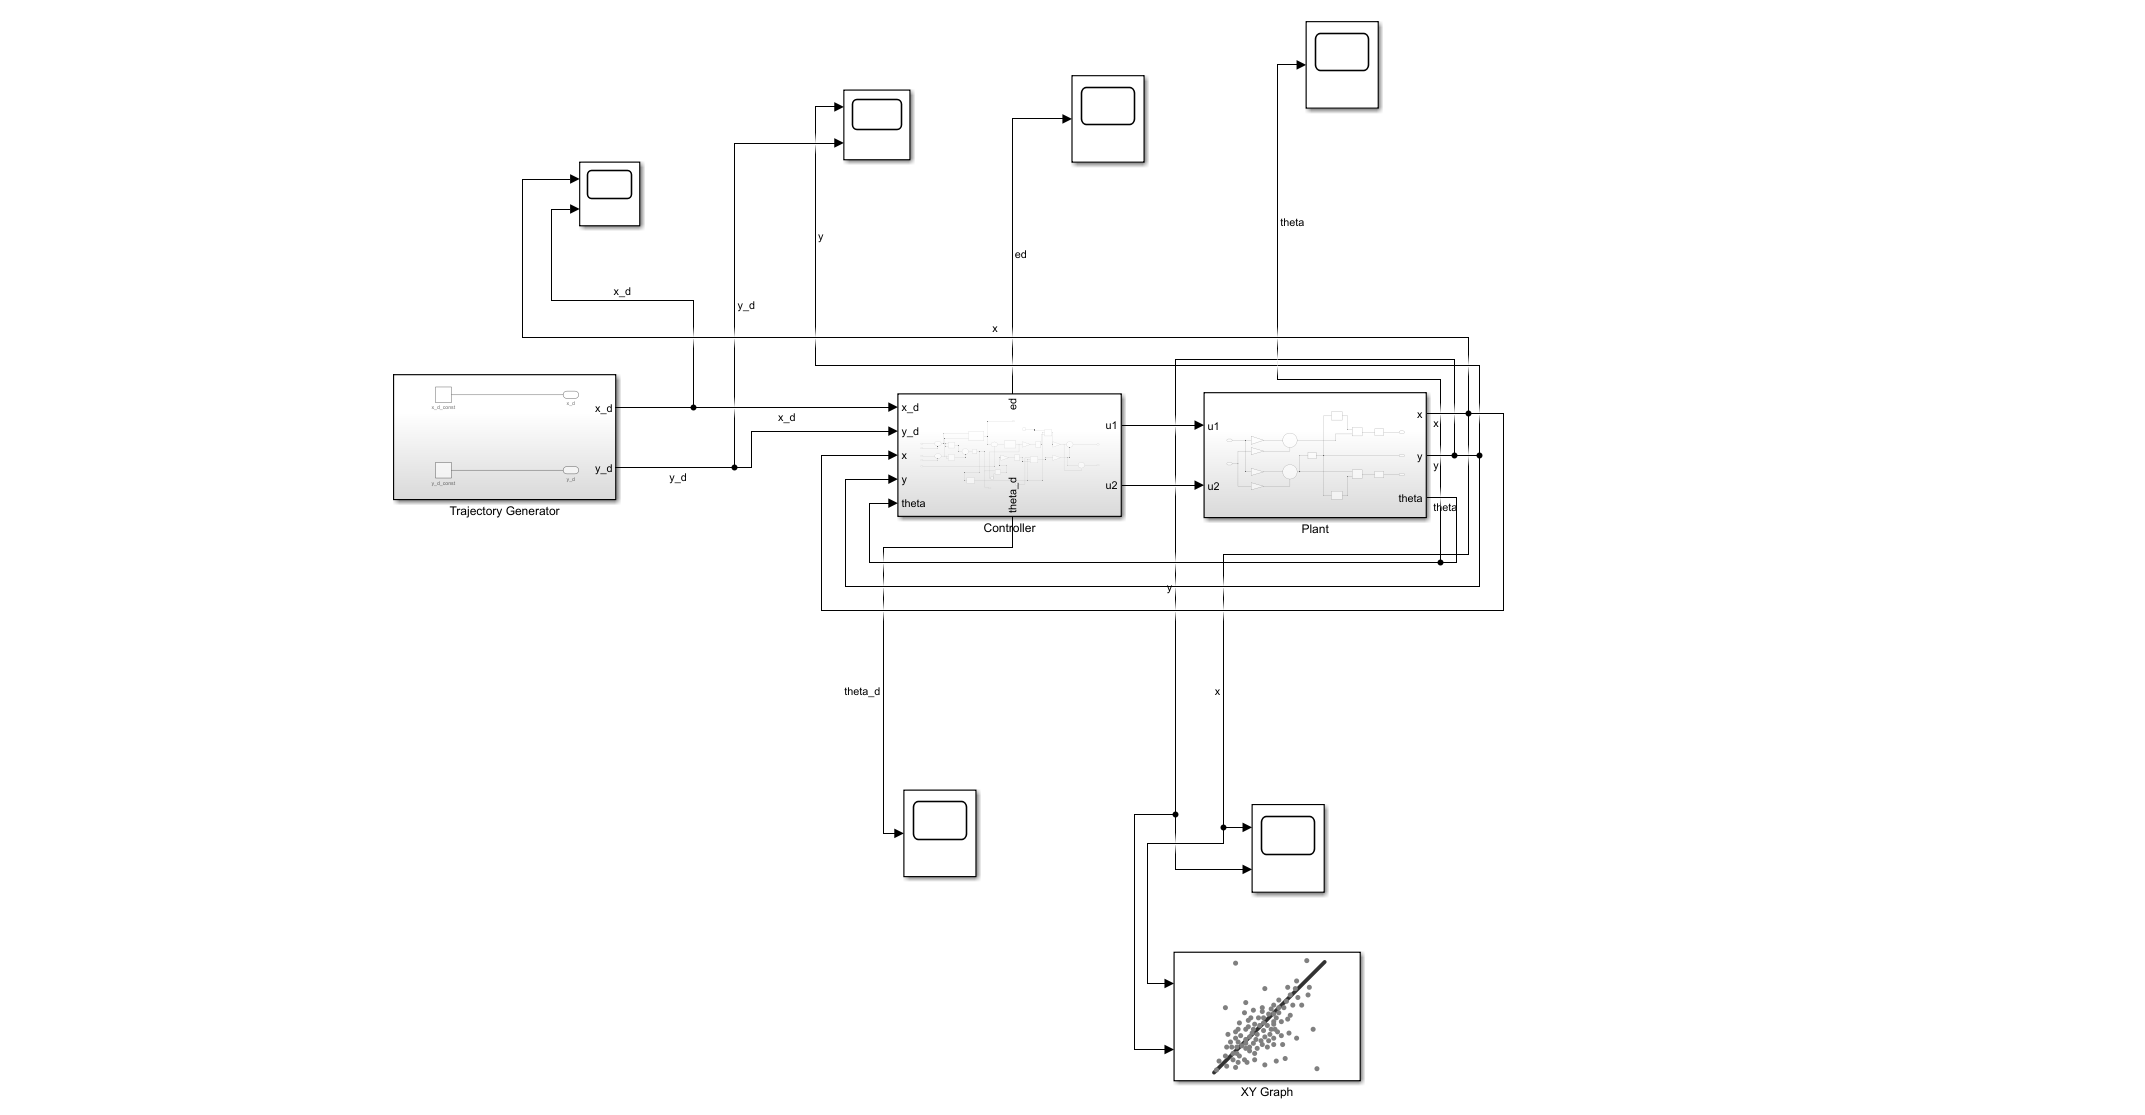
\includegraphics[width=1.0\textwidth]{chapter10/images/schema a blocchi.png}
    \caption{Implementazione del modello di controllo e del sistema dinamico in ambiente Simulink.}
    \label{fig:simulink_implementation}
\end{figure}

\section{Analisi dei Risultati}
Il controllore è stato validato su una traiettoria circolare (\( R=5 \) m, \( \omega_{ref}=0.3 \) rad/s). I risultati, mostrati in Figura \ref{fig:tracking_results}, dimostrano prestazioni eccellenti:

\begin{itemize}
    \item \textbf{Inseguimento (Grafico sx):} La sovrapposizione tra la traiettoria reale (blu) e quella di riferimento (nera tratteggiata) è perfetta. Non si evidenziano derive né overshoot significativi all'ingresso in curva.
    \item \textbf{Errore (Grafico alto dx):} L'errore di posizione si mantiene limitato entro \( \pm 2 \) cm (\( 0.02 \) m). Tale errore residuo oscillante è fisiologico per l'inseguimento di curve a velocità costante ma è del tutto trascurabile rispetto alla scala del movimento (5 m).
    \item \textbf{Ingressi (Grafico basso dx):} Le velocità delle ruote si stabilizzano sul valore teorico atteso \( u \approx 15 \) rad/s, mantenendosi ben lontane dai limiti di saturazione.
\end{itemize}

\begin{figure}[h]
    \centering
    % Assicurati che il percorso dell'immagine '2 punto.png' sia corretto
    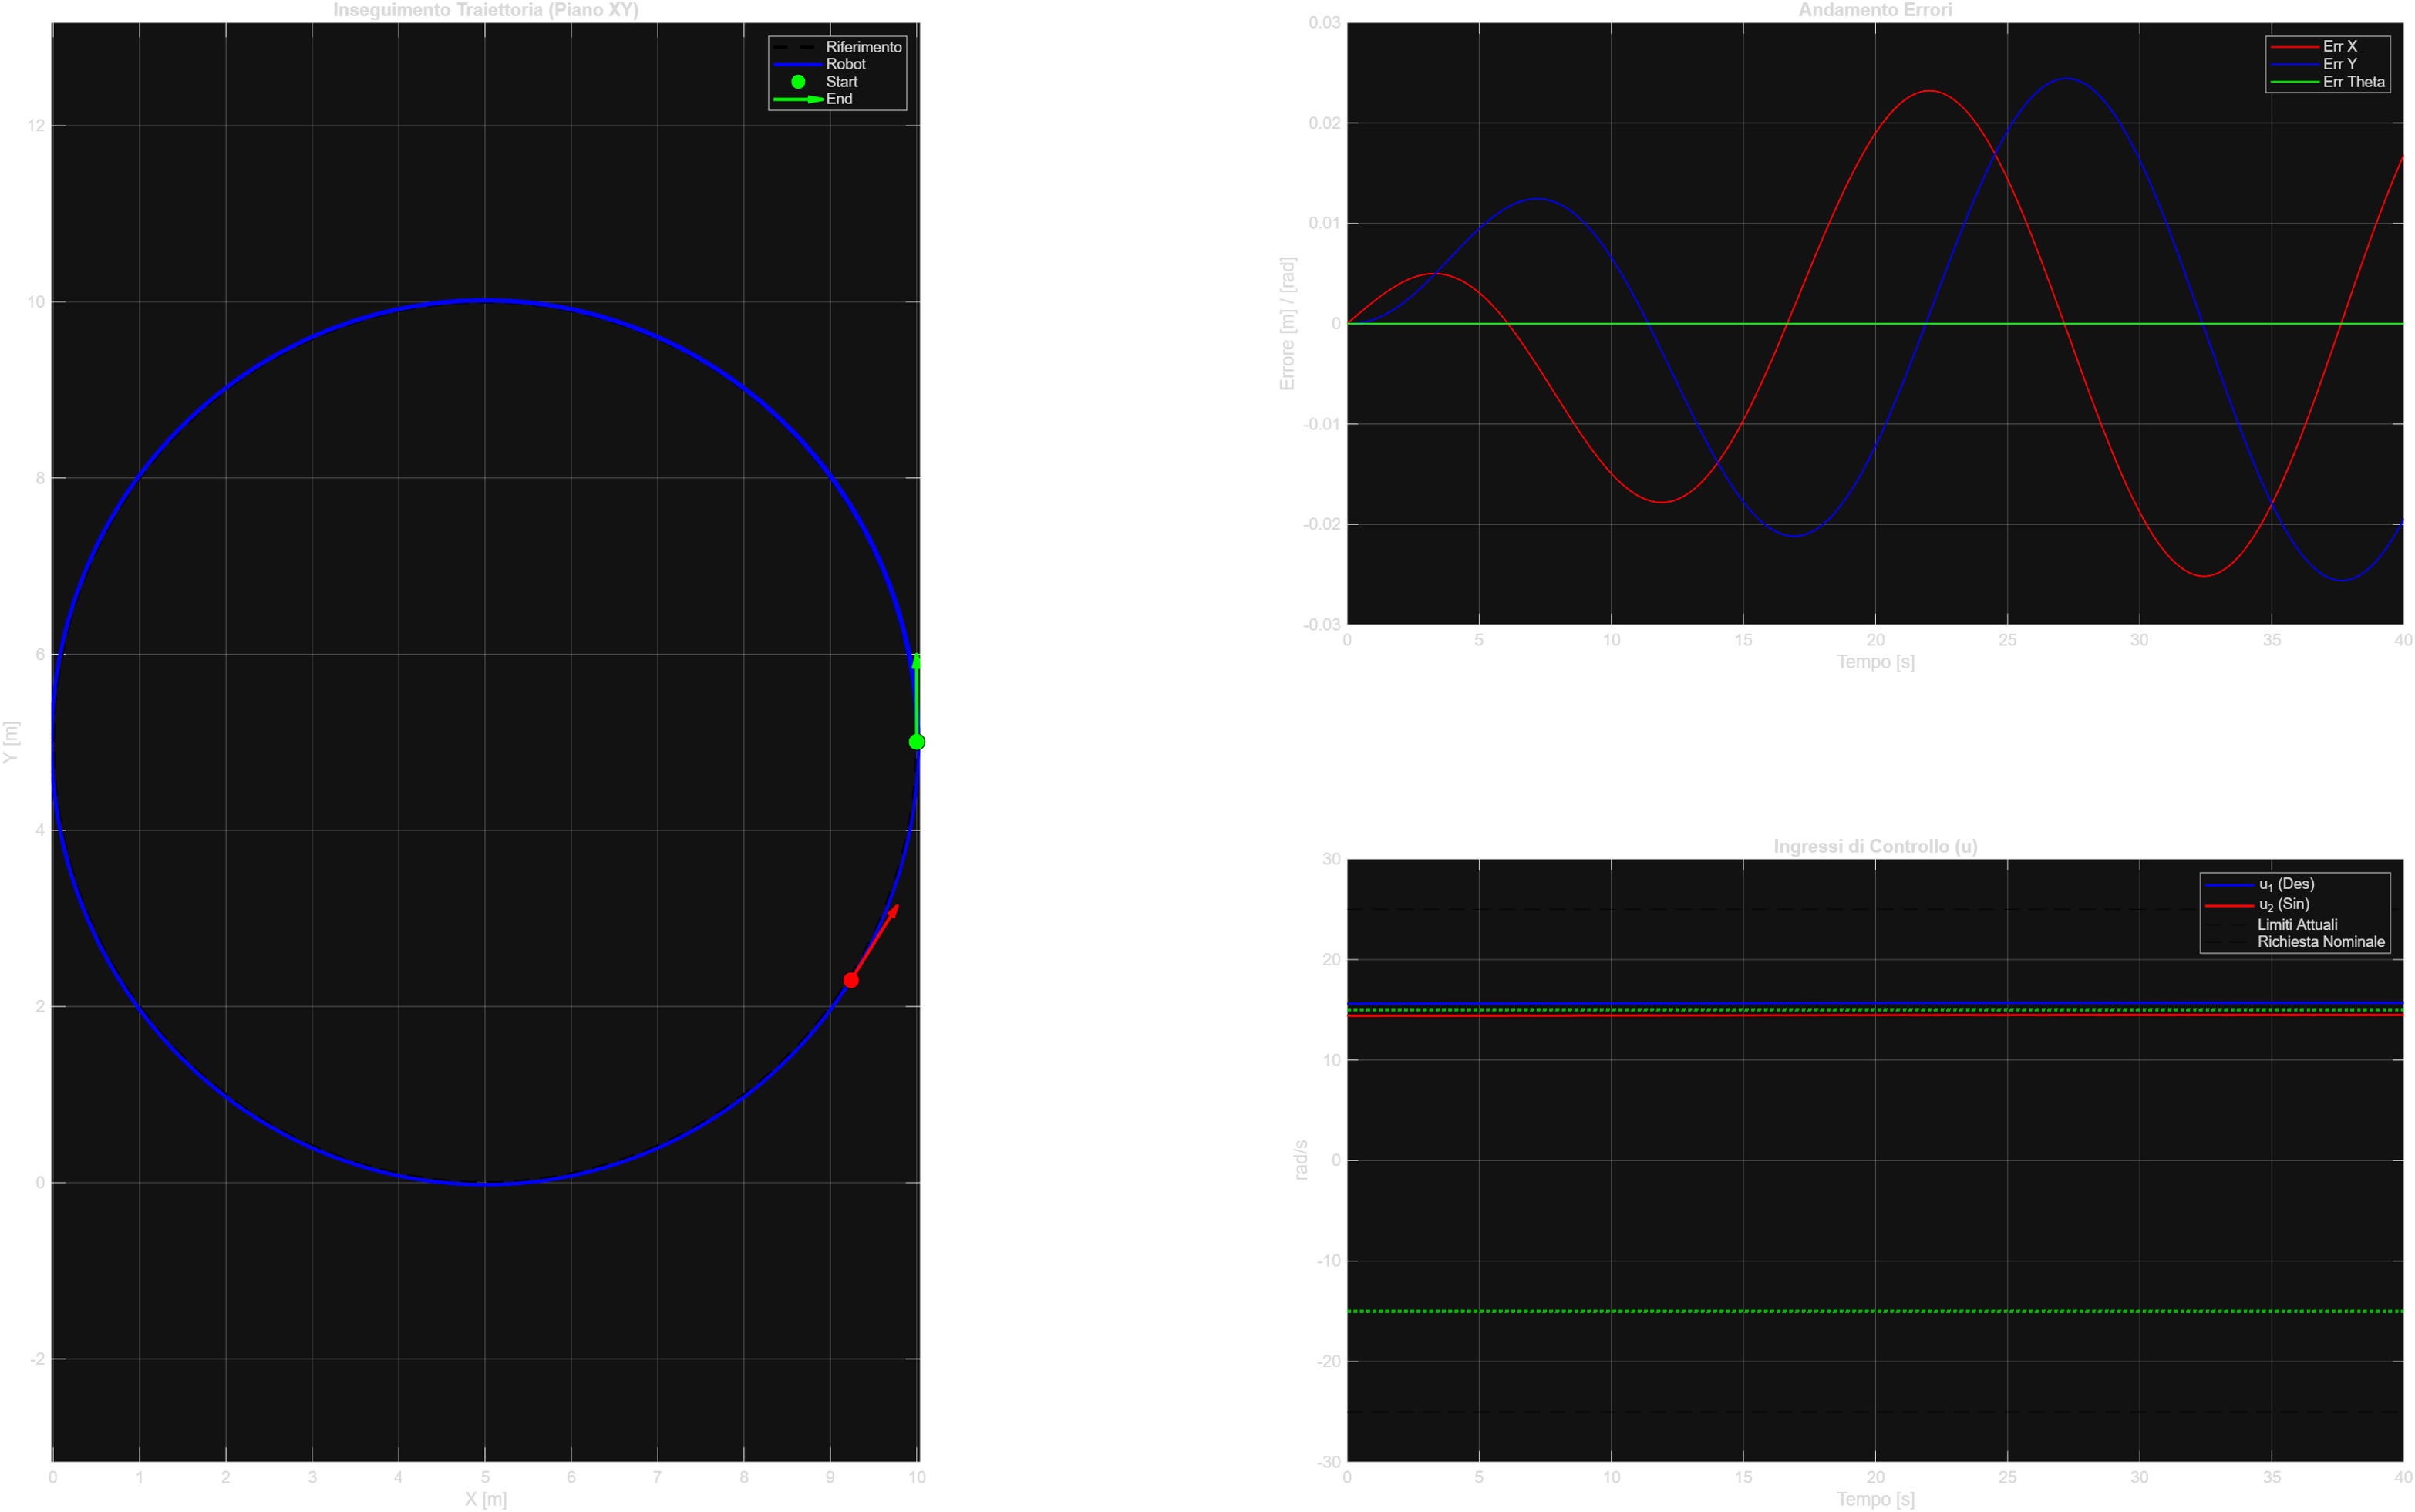
\includegraphics[width=1.0\textwidth]{chapter10/images/2 punto.png}
    \caption{Validazione del controllore: Traiettoria circolare, errori ed ingressi di controllo.}
    \label{fig:tracking_results}
\end{figure}

\section{Conclusioni Punto 2}
L'obiettivo di progettazione è stato raggiunto. Il controllore basato su feedback linearization garantisce un errore di tracking praticamente nullo e un comportamento degli attuatori dolce e realistico, fornendo una base solida per i successivi test di robustezza ai guasti.